%% 
%% Copyright 2019-2021 Elsevier Ltd
%% 
%% This file is part of the 'CAS Bundle'.
%% --------------------------------------
%% 
%% It may be distributed under the conditions of the LaTeX Project Public
%% License, either version 1.2 of this license or (at your option) any
%% later version.  The latest version of this license is in
%%    http://www.latex-project.org/lppl.txt
%% and version 1.2 or later is part of all distributions of LaTeX
%% version 1999/12/01 or later.
%% 
%% The list of all files belonging to the 'CAS Bundle' is
%% given in the file `manifest.txt'.
%% 
%% Template article for cas-dc documentclass for 
%% double column output.

\documentclass[a4paper]{cas-dc}

% If the frontmatter runs over more than one page
% use the longmktitle option.

%\documentclass[a4paper,fleqn,longmktitle]{cas-dc}

%\usepackage[numbers]{natbib}
%\usepackage[authoryear]{natbib}
\usepackage[authoryear,longnamesfirst]{natbib}

%%%Author macros
\def\tsc#1{\csdef{#1}{\textsc{\lowercase{#1}}\xspace}}
\tsc{WGM}
\tsc{QE}
%%%

% Uncomment and use as if needed
%\newtheorem{theorem}{Theorem}
%\newtheorem{lemma}[theorem]{Lemma}
%\newdefinition{rmk}{Remark}
%\newproof{pf}{Proof}
%\newproof{pot}{Proof of Theorem \ref{thm}}

\begin{document}
\let\WriteBookmarks\relax
\def\floatpagepagefraction{1}
\def\textpagefraction{.001}

% Short title
\shorttitle{Short title}    

% Short author
\shortauthors{Short author}  

% Main title of the paper
\title [mode = title]{Diagnosing autism spectrum disorders based on self-attention mechanism and dynamic functional connectivity}  

% Title footnote mark
% eg: \tnotemark[1]
%\tnotemark[1] 

% Title footnote 1.
% eg: \tnotetext[1]{Title footnote text}
%\tnotetext[1]{<Title footnote text>} 	% 文末注释

% First author
%
% Options: Use if required
% eg: \author[1,3]{Author Name}[type=editor,
%       style=chinese,
%       auid=000,
%       bioid=1,
%       prefix=Sir,
%     
%
%=0000-0000-0000-0000,
%       facebook=<facebook id>,
%       twitter=<twitter id>,
%       linkedin=<linkedin id>,
%       gplus=<gplus id>]

\author[1]{Libiao Chen}



% Footnote of the first author
%\fnmark[Model building]

% Email id of the first author
\ead{chenlb318@emails.bjut.edu.cn}

% URL of the first author
%\ead[url]{<URL>}

% Credit authorship
% eg: \credit{Conceptualization of this study, Methodology, Software}
\credit{Methodology}

% Address/affiliation
\affiliation[1]{organization={Beijing University of Technology},
            %addressline={}, 
            city={Beijing},
%          citysep={}, % Uncomment if no comma needed between city and postcode
            postcode={100000}, 
           % state={},
            country={China}}

\author[1]{Sizhe Wang}

% Footnote of the second author
\fnmark[1]

% Email id of the second author
\ead{wangzishe@qq.com}

% URL of the second author
%\ead[url]{}

% Credit authorship
\credit{Software}

\author[1]{Zhenyu Wei}
\ead{weizhenyu@qq.com}
\credit{Software2}
\fnmark[1]

\author[1]{Yaoqing Zhang}
\ead{zhangyaoqing@qq.com}
\credit{Software3}

\author[1]{Mengzhu Luo}
\ead{luomengzhu@qq.com}
\credit{Software4}

\author[1]{Yi Liang}
\ead{liangyin@qq.com}
\credit{Software5}
% Corresponding author indication
\cormark[1]

% Address/affiliation
%\affiliation[2]{organization={Beijing University of Technology},
%	addressline={}, 
%	city={Beijing},
%	%          citysep={}, % Uncomment if no comma needed between city and postcode
%	postcode={100000}, 
%	state={},
%	country={China}}

% Corresponding author text
\cortext[1]{Corresponding author}

% Footnote text
\fntext[1]{Second Author and Third Author contribute equally to this work.}
%\fntext[2]{fntext 2}

% For a title note without a number/mark
%\nonumnote{}

% Here goes the abstract
\begin{abstract}
Autism spectrum disorder (ASD) is a severe developmental illness that can severely impair the social abilities of those affected. Previous research has demonstrated impairments in functional brain connection in ASD patients. This paper proposes a strategy for categorizing ASD based on the self-attention mechanism. Patients' dynamic functional connectivity (dFC) data were collected using sliding windows, and Kendall's rank correlation coefficient was utilized to extract the features. A structure based on the multi-head self-attention mechanism is utilized to identify ASD using selected highly discriminative features. Then, using ten-fold cross-validation and inter-site cross-validation on the ABIDE database, we evaluated the model's performance and compared it to other published approaches. In ten-fold cross-validation, this model achieved an average accuracy of 76.22\% and an AUC of 0.8132, while in site cross-validation, it achieved an average accuracy of 76.71\% and an AUC of 0.7957. In addition, the 30 functional connections most likely to lead to ASD are shown based on the results of the feature ranking and the results showed that the superior frontal gyrus and middle temporal gyrus have the greatest impact.
\end{abstract}

% Use if graphical abstract is present
%\begin{graphicalabstract}
%\includegraphics{}
%\end{graphicalabstract}

% Research highlights
\begin{highlights}
\item A novel model employing the self-attention mechanism on dynamic functional connectivity is proposed for the classification of ASD. Based on the findings of feature rating, the most distinctive brain area connections are also displayed.

\item In this paper, sliding windows are used to acquire dynamic functional connectivity between brain regions, and Kendall rank correlation coefficients are employed for feature selection and as a basis for determining the most discriminative brain region connection. The multi-head self-attention mechanism was employed in conjunction with feedforward neural networks and residual networks to extract higher-order features from the data and discriminate ASDs.

\item This model obtained an average accuracy of 76.22\% and an AUC of 0.8132 on the ABIDE dataset, achieving excellent outcomes among similar studies. The superior frontal gyrus and middle temporal gyrus are identified as the brain regions most likely to cause ASD. 
\end{highlights}

% Keywords
% Each keyword is seperated by \sep
\begin{keywords}
 ASD\sep Self-Attention\sep dFC\sep rs-fMRI \sep Kendall
\end{keywords}

\maketitle

% Main text
\section{Introduction}\label{Introduction}
Autism spectrum disorder (ASD) is a neurodevelopmental illness characterized by social interaction deficiencies, communication deficits, restricted interests, and repetitive, stereotypical behaviors. These deficiencies impact the learning and living of autistic patients, causing them to have considerable difficulties expressing their needs, comprehending others, and maintaining relationships, resulting in aberrant behaviors. In 2021, the CDC estimated that 1 in 44 U.S. children had been diagnosed with ASD (Matthew J. Maenner,2021). Consequently, early detection of ASD is essential. However, the etiology and pathophysiology of ASD remain uncertain. Thus, the identification and diagnosis of ASD are now restricted to symptomatological observations and clinical experiences. In recent years, it has become widely accepted that mental diseases, such as ASD, are caused by aberrant connections between large-scale brain networks, and neuroimaging-based diagnostic approaches have become an essential research direction.

Resting-state functional magnetic resonance imaging (rs-fMRI) is a non-radioactive, non-invasive means of detecting functional brain activity. It depicts the variations in the Blood Oxygen Level Dependent (BOLD)  signals that occur naturally when a subject is not engaged in a specific task. (Neil D. Woodward,2015)  found that neurological and psychiatric disorders are characterized by alterations in the interactions between rs-fMRI, suggesting that the entire brain should be considered a holistic network. (Christopher S. Monk,2009) found that ASD altered the intrinsic connectivity of subjects' brain networks. Previous studies have typically used functional connectivity (FC) analysis to quantify correlations between brain regions. They have shown excellent results in various psychiatric disorders, such as Alzheimer's Disease(Ronghui Ju,2019) and Major depressive disorder(Ling-Li Zeng,2012). Thus we can build FC utilizing the activity of all brain regions and identify a decline in brain function by comparing the connectivity of specific brain regions between ASD patients and healthy individuals through rs-fMRI data, which is proven to be effective(Neil D. Woodward,2015), (Michal Assaf,2010).  

Machine learning methods are widely used for classification tasks with their efficient performance and advanced methods. (Alexandre Abraham, 2017) utilized support vector machine (SVM) on 871 samples and attained a cross-validation accuracy of 67\% between sites. (Eman Ismail,2022) proposed a hybrid ensemble-based classification (HEC-ASD) model, which obtained 80\% classification accuracy using random forest. 

Due to the single-layer structure of these traditional machine learning methods, it is difficult to acquire high-level information from complex features. Deep learning algorithms learn higher dimensional information by stacking layers to address these drawbacks. (Yin Liang,2021) proposed a novel convolutional neural network combined with a prototype learning (CNNPL) framework and got excellent results. (Ronghui Ju,2019) divided the dataset for each subject into 30 independent components (IC) and used stacked autoencoder (SAE) to obtain 87.21\% accuracy on a small sample set. Long short-term memory (LSTM) were used by(J. Kittler,2017)  to obtain the temporal data from rs-fMRI and eventually achieved 68.5\% accuracy. 

Although deep learning algorithms offers superior performance, most current research ignores the dynamic changes between FCs. Instead, they assume that the subject's brain state remains constant during the test (5-30 minutes), which is proven to be inaccurate (Vince D. Calhoun,2014). Dynamic FC (dFC) based on the sliding window has become a new research direction. The sliding window method separates the time series into many independent and overlapping windows. By evaluating the discrepancies between different windows, the fluctuations of the sample on the time series are obtained. (Antonis D. Savva, 2019) investigates the effect of different window lengths on model performance. (Geert Litjens, 2017) used convolutional neural networks and self-attention mechanisms to achieve outstanding outcomes. Compared to static FC, dFC can capture oscillations in the BOLD signal, which unquestionably contributes extra information to the discrimination of ASD.

%Methods for measuring correlations between brain regions are essential to building FC network. The most common way to measure the correlation between each pair of brain regions is using the Pearson correlation coefficient. In addition, Spearman's rank correlation coefficient (reference) and high-order FC(HOFC)(reference) were also used.

As time series are partitioned into several overlapping windows, the sliding window exacerbates the conflict among small sample sizes, high dimensionality, big parameters while simultaneously capturing more information. However, numerous recent investigations have demonstrated the sparseness of brain activity. Thus, the network model is more susceptible to noise interference and overfitting. To reduce the interference of noise while acquiring more discriminative features, (A. R. J. Fredo, 2018) employed conditional random forest to reduce the dimensionality of the FC matrix and used random forest to test the classification accuracy of each dimension. (Xinyu Guo, 2017) chose features from many trained sparse auto-encoders (SAE) with strong discriminating power. (Yin Liang, 2021) ranked the characteristics using Kendall's rank correlation coefficient and retrieved more discriminative features without altering the raw data.

The self-attention (SA) mechanism is derived from the Transformer(Ashish Vaswani,2017) in natural language processing. It has now replaced CNN to obtain superior results in various computer vision fields because it can combine global information and concentrate more on critical regions than CNN, which can only focus on local information within the convolution kernel. Meanwhile, parallelism makes SA more computationally efficient than RNN and LSTM. However, the self-attention mechanism lacks attention to temporal order, which means changing the input order does not affect the output. Transformer alleviates this problem by adding positional encoding information to the raw data without increasing the data's dimensionality. Recent research has focused on using SA to identify brain illnesses using rs-fMRI data(Jeongjae Kim,2022), (Geert Litjens,2017).The multi-head self-attention (MSA) mechanism computes the self-attention formulas in many subspaces in parallel and stitches the final results together in order to capture the data in distinct spaces.

This paper proposed a method for diagnosing ASD based on dFC and MSA mechanism. Initially, the raw data is partitioned into many independent windows on the time series using the sliding window approach. For each window, the correlation between brain regions is assessed using Pearson correlation coefficients and constructed into feature vectors, then the feature vectors of all windows are combined to form the input feature matrix for each sample. To overcome the problem of high dimensionality, feature extraction is performed using the Kendall rank correlation coefficient. Through multi-head self-attention layers that combine feedforward neural networks and residual networks, higher-order characteristics are extracted, and then ASD is dichotomized through a fully connected layer. On the ABIDE dataset, the performance of the model is displayed and compared to other models using ten-fold cross-validation. Meanwhile, the generalization of the model is explained by inter-site cross-validation. Finally, considering the feature ranking results of all windows together, we ranked the functional connectivity of brain regions most likely to cause autism. The main contributions of our work are as follows.
\begin{enumerate}[a)]
	\item A novel model employing the self-attention mechanism on dynamic functional connectivity is proposed for the classification of ASD. Based on the findings of feature rating, the most distinctive brain area connections are also displayed.
	\item In this paper, sliding windows are used to acquire dynamic functional connectivity between brain regions, and Kendall rank correlation coefficients are employed for feature selection and as a basis for determining the most discriminative brain region connection. The multi-head self-attention mechanism was employed in conjunction with feedforward neural networks and residual networks to extract higher-order features from the data and discriminate ASDs.
	\item This model obtained an average accuracy of 76.22\% and an AUC of 0.8132 on the ABIDE dataset, achieving excellent outcomes among similar studies. The superior frontal gyrus and middle temporal gyrus are identified as the brain regions most likely to cause ASD.
\end{enumerate}  
The rest paper is organized as follows. In the "Materials and Methods" section, we first describe how to preprocess raw data and generate dynamic functional connectivity using sliding windows. We then propose a feature reduction method based on Kendall's rank correlation coefficients and classify ASDs using a model based on the multi-head self-attention mechanism. In the "Result" section, we discuss the experimental results, compare them to other models, and offer the 30 functional connections that may contribute to ASDs. In the "Conclusion" section, we provide a paper summary.
% Numbered list
% Use the style of numbering in square brackets.
% If nothing is used, default style will be taken.


% Unnumbered list
%\begin{itemize}
%\item 
%\item 
%\item 
%\end{itemize}  

% Description list
%\begin{description}
%\item[]
%\item[] 
%\item[] 
%\end{description}  

% Figure
%\begin{figure}[<options>]
%	\centering
%		\includegraphics[<options>]{}
%	  \caption{}\label{fig1}
%\end{figure}




% Uncomment and use as the case may be
%\begin{theorem} 
%\end{theorem}

% Uncomment and use as the case may be
%\begin{lemma} 
%\end{lemma}

%% The Appendices part is started with the command \appendix;
%% appendix sections are then done as normal sections
%% \appendix

\section{Materials and Methods}\label{Materials and Methods}
\subsection{Data and preprocessing}
In this study, we use resting-state fMRI data obtained from ABIDE database. The ABIDE dataset comprises structural and functional brain imaging data from 17 international imaging locations that work together to capture and exchange neuroimaging data from 539 people with ASD and 573 healthy controls (HC). The 1112 data included a substantial amount of phenotypic data together with structural and static functional MRI data. However, using the complete sample data to establish dynamic functional connections may result in different input sizes due to the varying collecting periods $T$ across sites. Consequently, we dropped some samples with too short a collection time and shortened those with a longer collection time. After taking into account the sample size and the time length of the sample, $T$ was set to 146. We also excluded samples missing some data. For each site following removal, sample information is shown in Table \ref{Table1}.

\begin{table}[]
\caption{Site information used in this paper}\label{Table1}
\begin{tabular*}{\tblwidth}{@{}cccc@{}}
\toprule
  \textbf{Sites} & \textbf{Size} & \textbf{Sample(ASD/HC)} & \textbf{Gender(M/F)} \\ % Table header row
\midrule
CALTHCH                 & 20                           & 8/12          & 14/6               \\
CMU                     & 1                            & 1/0           & 1/0                    \\
KKI                     & 34                           & 10/24          & 26/8                 \\
LEUVEN\_1               & 29                           & 14/15          & 29/0                \\
LEUVEN\_2               & 31                           & 13/18          & 24/7                \\
NYU                     & 166                          & 71/95          & 132/34              \\
OLIN                    & 25                           & 14/11          & 20/5                \\
PITT                    & 32                           & 17/15          & 25/7                \\
SBL                     & 8                            & 3/5           & 8/0                \\
SDSU                    & 27                           & 9/18          & 21/6                \\
STANFORD                & 36                           & 17/19          & 28/8                \\
TRINITY                 & 43                           & 21/22          & 43/0                \\
UM\_1                   & 82                           & 36/46          & 59/23               \\
UM\_2                   & 31                           & 12/19          & 29/2                 \\
USM                     & 61                           & 38/23          & 61/0                \\
YALE                    & 48                           & 22/26          & 34/14               \\
TOTAL                   & 674                          & 306/368         & 554/120            \\
\bottomrule
\end{tabular*}
\end{table}
To facilitate the research and expansion, we use the preprocessing version of ABIDE dataset and use Anatomical Automatic Labeling (AAL) template to classify brain regions. AAL is provided by the Montreal Neurological Institute (MNI). It divides the whole brain region of interest (ROI) into 116 regions, of which 90 belong to the brain and 26 to the cerebellum. The sample data for each subject is arranged as a table of $T\times R$, where $R$ is the number of ROI. Each value represents the average BOLD signal strength of all the voxels in a given ROI at that particular time.

The BOLD signal in the brain region will be erroneous during data collection due to subject head movement and instrument error. Thus the data must be pre-processed. The main steps include Time correction, Head motion realignment, Coregister, Normalize, Smooth, Detrend, Filter.

\begin{figure*}[t]
	\centering
	\label{Fig1}
	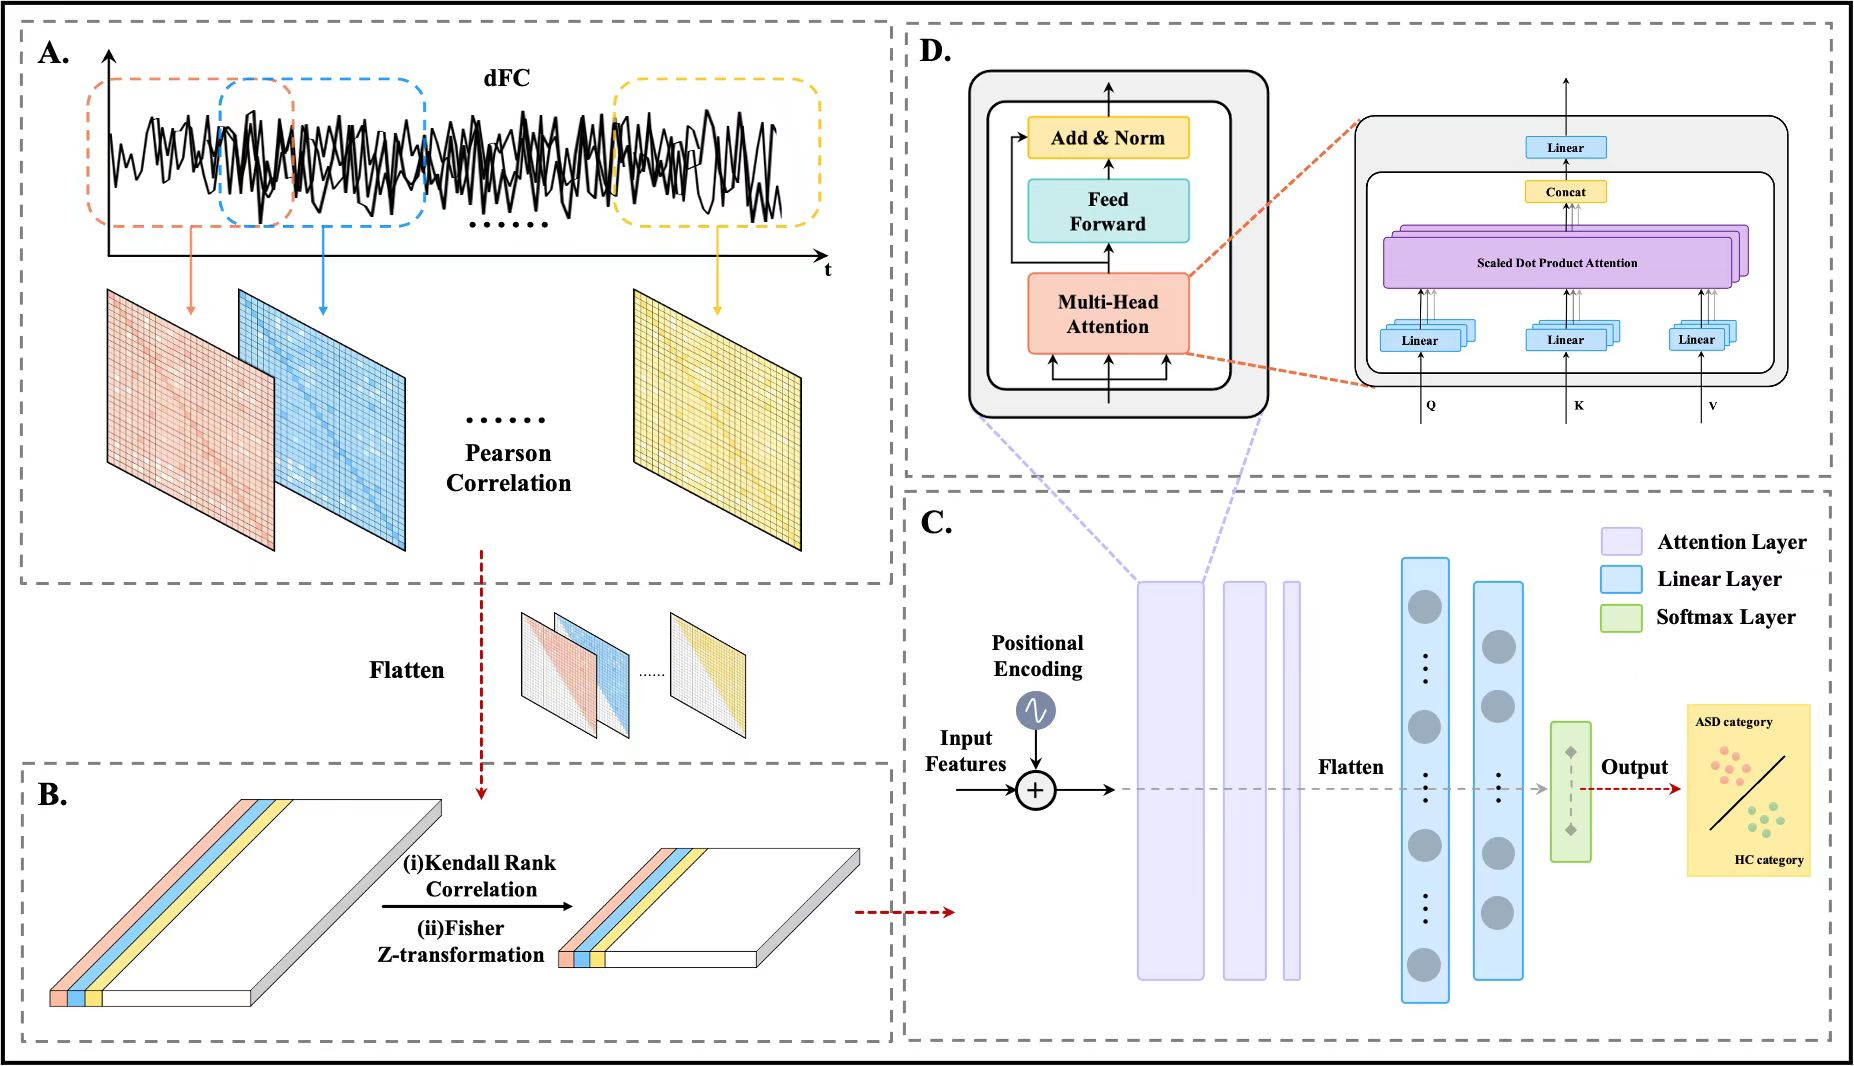
\includegraphics[width=\textwidth]{model.jpg}
	\caption{Flowchart of this paper. Box A shows dynamic functional connection acquisition. Box B shows feature extraction and normalization. Box C shows stacking multi-head self-attention layers with fully connected layers for classification. Box D shows the multi-head self-attention layer structure.}
\end{figure*} 

\subsection{Construction of Brain Functional Network}
The complete flow chart of the model is shown in Figure \ref{Fig1}. This section will explain how to generate dynamic brain functional connectivity networks using preprocessed data. 
\paragraph{silding windows method}~{}
\newline
\indent Initially, assume that a window of fixed length $l$ moves through the time series of data at a constant step $s$. The window partitions the entire time series into many overlapping but mutually distinct subsequences. The sliding window method necessitates the selection of parameters such as window length and window step beforehand. The window length defines the balance between temporal resolution and estimating precision(reference). Smaller window sizes are more sensitive to changes in time, but they add more noise, which makes the contradiction between small sample sizes and high dimensionality worse. Referring to the findings of previous studies, we define the window length $l$ = 30 and the step size $s$ = 1, the preprocessed data is divided into $N$ ($N = \left \lfloor \frac{T - l}{s} \right \rfloor + 1$)separate windows.
\paragraph{Pearson's correlation coefficient}~{}
\newline
\indent Brain connections create a sophisticated network that enables a variety of high-level tasks. Pearson's correlation coefficient is widely used to establish functional connectivity between brain regions. The Pearson correlation coefficient assumes that the data follow a normal distribution so we conducted the Shapiro-Wilk test on randomly selected regions of the brain for each sample to assess whether the data followed a normal distribution. The results indicated that $P=0.421\pm 0.295>0.05$ and $W=0.989\pm 0.004$, thus we could not reject the null hypothesis at the 0.05 level of significance, and the time series followed a normal distribution.

After checking, for each window $W_n$, We define $x_{i}(t)$,$x_{j}(t)$ as the rs-fMRI signals of two brain regions $i$ and $j$ at time point $t$($t = 1,2,...,l$).The $FC_{ij}$ can be defined as,
\begin{equation}
	FC_{ij}=\frac{\sum_{t=1}^{l}(x_{i}(t)-\bar{x_{i}})(x_{j}(t)-\bar{x_{j}})}{\sqrt{\sum_{t=1}^{l}(x_{i}(t)-\bar{x_{i}})^2}\sqrt{\sum_{t=1}^{l}(x_{j}(t)-\bar{x_{j}})^2}}
\end{equation}
where $\bar{x{i}}$ and $\bar{x{j}}$ represent the mean of rs-fMRI in brain regions $i$ and $j$.For AAL with 116 ROIs, the calculation between every two regions will end up with 6670 ($6670=\frac{116\times115}{2}$) features. The feature vector of each window consists of all 6670 features. The feature space of each sample is derived by sewing together the feature vectors of all windows. The shape of the feature space can be expressed as $N\times 6670$.
\subsection{Feature Ranking by Dynamic Kendall Rank Correlation}
Compared with static FC, dFC acquires more information while making the problem of high feature dimensionality more significant. Reducing the number of features by retaining more discriminative features can effectively reduce redundant noise in the data and improve computing efficiency. In this paper, we used the Kendall rank correlation coefficient, which measures the relevance of each feature with the classification by a distribution-free test of independence between two variables.We apply it separately to each window and combine the rating results to determine the final set of selected attributes. 

Assume that $m$ and $n$ correspondingly represent the number of ASD patients group and HC group. For the $i$-th window of all samples, Let $z_{jk}$ denote the $j$-th feature of the $k$-th sample and $y_i$ denote the class label of this sample. For $z_{jp}$ from the ASD patient group and $z_{jq}$ from the HC group, the $i$-th window's Kendall tau correlation coefficient of the functional connectivity feature $j$ can be defined as:
\begin{equation}
	\tau_{ij} = \frac{n_c - n_d}{m \times n}
\end{equation}
where $n_c$ and $n_d$ denote the numbers of concordant and discordant pairs. It is a concordant pair when
\begin{equation}
	sgn(z_{jp} - z_{jq}) = sgn(y_p-y_q)
\end{equation}
where sgn() is a signum function. Correspondingly, it is a disconcordant pair when
\begin{equation}
	sgn(z_{jp} - z_{jq}) = -sgn(y_p-y_q)
\end{equation}

The absolute value of each $\tau_{ij}$ can characterize the ability of feature $j$ to detect ASD in the $i-th$ window. The greater the absolute value, the higher the discriminating power. To represent the combined discriminative capacity of feature $j$ in all windows, the discriminative power of feature $j$ against ASD in dynamic functional connectivity was calculated by averaging the correlation coefficient $\tau_{ij}$ of feature $j$ across all windows, which can be expressed as:
\begin{equation}
	\tau_{j} =  \frac{1}{N}\sum_{i=1}^{N}\tau_{ij}
\end{equation}

After calculating the average correlation coefficient of each features, we rank them from highest to lowest and then select the top $C$ ($C\leq6670$) features. The shape of data changed from $N\times 6670$ to $N\times C$. The value of $C$ is proportional to the sparsity of functional brain connections; a smaller $C$ reduces the effect of noise on categorization but may result in a lack of meaningful information. 

The results of feature ranking can suggest which features are more likely to be linked to ASD. Note that each feature was calculated to reflect a correlation between two brain areas. Thus, the ranking data can be used to interpret the functional connections most likely to result in ASD.
\subsection{Classification based on Multi-Head Self-Attention}
\paragraph{Position Encoding}~{}
\newline
\indent By assigning different weights to inputs, self-attention mechanism can assist models in comprehending global relationships between inputs and focusing on more essential information. However, while its parallelism increases the efficiency of the model's operations, it disregards the order of the model's inputs, which means changing the order of the model's inputs has no effect on the model's output. This is certainly a loss of information for models that will be fed with continuous windows. 
To tackle this issue, we employ the same position encoding strategy as Transformer, appending position information to the data before it enters the self-attention layer. Define $n_i(i=1,2,..., N)$ to represent each independent window, and $c_j(j=1,2..., C)$ to represent the index of each window's feature vector. The sine and cosine functions of various frequencies determine the position encoding PE, which can be represented as,
\begin{equation}
	PE_{(c_i,2k)}=sin(c_i/10000^{2k/C})
\end{equation}
\begin{equation}
	PE_{(c_i,2k)}=cos(c_i/10000^{2k/C})
\end{equation}
Where $k(k<\frac{j}{2})$ is used to map to index $j$. Then, $PE$ is added to each sample's data to provide positional encoding information without expanding the data's dimensions.

\paragraph{Self-Attention Layer}~{}
\newline
\indent We use $N$ windows as the input and $C$ as the dimension of each input. The vector $I = (I_0, I_1,..., I_N)$ are first fed into the self-attention layer, and then three matrix $Q$,$K$,$V$ are defined as
\begin{equation}
	Q = IW_Q
\end{equation}
\begin{equation}
	K = IW_K
\end{equation}
\begin{equation}
	V = IW_V
\end{equation}
The weights of the input vectors are then defined as
\begin{equation}
	\alpha = Softmax(\frac{QK^T}{\sqrt{d_k}})
\end{equation}
Finally, the output matrix O is defined as
\begin{equation}
	O = \alpha V
\end{equation}

Due to the complexity of brain functional connectivity, we used the multi-head self-attention layer to obtain rich information on functional connectivity. The multi-head self-attention layer creates $H$ subspaces, executes the self-attention function on each subspace in parallel, and then combines the results of all subspaces as output.

Furthermore, to extract higher-order features, we stack multiple layers of the multi-head self-attention layer while making the dimension $d_v$ of the matrix $V$ smaller than the dimension $d_{qk}$ of matrices $Q$ and $K$ for dimensionality reduction, so the output dimension of the multi-head self-attention layer can be expressed as $N\times Hd_v$.

We incorporate feedforward neural networks between the multi-headed self-attention layers to achieve nonlinear transformation of features. First, the output of the self-attention layer is transferred to a higher dimension so that information can be combined to produce deeper associations. Then, the higher-dimensional output is reduced to the original dimension in order to eliminate combinations with low discriminatory power.

In addition, a residual network is added to the feedforward neural network to avoid the gradient vanishing and speed up the model's training. Moreover, a Dropout layer is also utilized to prevent overfitting of the model.

Following the preceding operations, the data will be reduced to two dimensions by the fully connected layer(FC), and the model output will be generated by Softmax. The loss function used in the model is the cross-entropy loss function combined with the L2 regularized loss function. The optimizer used is SGD.
\section{Result}
In this section, we analyze the effect of the number of features chosen and the number of heads of the multi-head self-attention layers, compare the method described in this research to previous models, and demonstrate the brain area connections most likely to induce ASD.
\subsection{Impact of feature numbers and head numbers to classification results}
Due to the sparsity of brain connections and the high dimensionality, the number of characteristics chosen becomes a key determinant of classification outcomes. In order to determine the optimal value for the number of features, we trained the model utilizing the top 100, 512, 1024, 1600, and 6670 Kendall features, respectively. The conclusive results are shown in Table \ref{Table2}. We can see that the model performs best with 1024 features, and its accuracy increases by 8.92\% compared with no feature reduction, indicating that there is a great deal of noise in the raw data and that feature extraction is essential. To demonstrate the dependability of feature ranking, we randomly picked 1024 features for testing, and the results demonstrate that Kendall can not only minimize the data dimensionality but also select the most discriminative features in a very effective way.
\begin{table}[]
	\caption{Experimental results using 100, 512, 1024, 1600, and 6670 features as model inputs,(r) means random}\label{Table2}
	\begin{tabular*}{\tblwidth}{@{}ccccc@{}}
		\toprule
		\textbf{Number}& \textbf{Accuracy} & \textbf{Sensitivity} & \textbf{Specificity} & \textbf{AUC} \\ % Table header row
		\midrule
		100                                     & 0.7090              & 0.6453                & 0.7651                 & 0.7664           \\
		512                                     & 0.7448              & \textbf{0.7112}       & 0.7759                 & 0.8080           \\
		1024                                    & \textbf{0.7622}     & 0.6554                & 0.8458                 & \textbf{0.8132}  \\
		1024(r)                                 & 0.6045              & 0.2869                & 0.8426                 & 0.6162           \\
		1600                                    & 0.7463              & 0.6253                & 0.8490                 & 0.7930           \\
		6670                                    & 0.6716              & 0.4482                & \textbf{0.8583}        & 0.7034 \\
		\bottomrule
	\end{tabular*}
\end{table}
We also investigated the effect of the number of heads $H$ on model performance in the multi-head self-attention layers, and the experimental results are shown in Table \ref{Table3}.The model performed best at $H$ = 6, indicating that the functional brain connections contain a wealth of information. When the number of heads exceeds six, it is difficult for the number of samples to support the training of a high number of parameters, resulting in a decline in the model's efficacy.
\begin{table}[]
	\caption{Experimental results using 1,2,4,6,8 heads in multi-head self-attention layers}\label{Table3}
	\begin{tabular*}{\tblwidth}{@{}ccccc@{}}
		\toprule
		\textbf{Number}& \textbf{Accuracy} & \textbf{Sensitivity} & \textbf{Specificity} & \textbf{AUC} \\ % Table header row
		\midrule
		1                            & 0.7343                & 0.6465                   & 0.8123                   & 0.7996           \\
		2                             & 0.7507                & \textbf{0.6751}          & 0.8177                   & 0.8022           \\
		4                             & 0.7358                & 0.6190                   & 0.8315                   & 0.8028           \\
		6                             & \textbf{0.7622}       & 0.6554                   & \textbf{0.8458}          & \textbf{0.8132}  \\
		8                             & 0.7343                & 0.6039                   & 0.8451                   & 0.8040      \\
		\bottomrule
	\end{tabular*}
\end{table}
\subsection{Results presentation and model comparison}
The k-fold cross-validation can maximize the use of samples for model testing and is commonly employed on small sample datasets. This method divides all samples into $k$ folds, selects $k-1$ folds as the training set and 1 fold as the test set for training, and repeats $k$ times to classify each fold as the test set.
% In this paper, we evaluate the classification capacity of the model using ten-fold cross-validation, as was done in the vast majority of prior research.

Multiple models were implemented for comparison. The first model is a logistic regression (LR) with L2 regularization terms and 1000 maximum iterations. Then, a support vector machine based on the rbf kernel function is created with the penalty value set to 1. Both LR and SVM are trained using dFC data, and Kendall rank correlation coefficients are used for feature extraction.

We have also implemented the three deep learning algorithms listed below. A model that extracts gradually high-level features by stacking 2D-CNNs, employing ELU activation functions and L2 regular terms with a value of 0.005(refer).A model that imitates the LSTM model in (refer) and employs a two-layer LSTM to extract information from time series following feature extraction.mA model that employs CNN for feature extraction, LSTM for temporal information extraction, a single self-attention layer for higher-order feature extraction, and a fully connected layer for classification(refer).

We chose accuracy, sensitivity, specificity and AUC as the evaluation indicators. The results are shown in Table \ref{Table4}. The model proposed in this paper achieves an average accuracy of 76.22\% in ten folds, while SEN, F1 score and AUC all obtain better results than those of similar models, which indicates that our model has excellent classification performance. 
\begin{table}[]
	\caption{Comparison of the classification performances between our method and other methods}\label{Table4}
	\begin{tabular*}{\tblwidth}{@{}ccccc@{}}
		\toprule
		\textbf{Model}& \textbf{Accuracy} & \textbf{Sensitivity} & \textbf{Specificity} & \textbf{AUC} \\ % Table header row
		\midrule
		LR             & 0.7272                   & 0.6723                   & 0.7771                   & 0.7247                   \\
		SVM            & 0.7404                   & 0.6134                   & \textbf{0.8514}          & 0.7324                   \\
		CNN         & 0.6836                   & 0.5847                   & 0.7628                   & 0.6202                   \\
		LSTM           & 0.7164                   & 0.5966                   & 0.8151                   & 0.7610                   \\
		CLAttention    & 0.7448                   & 0.6369                   & 0.8356                   & 0.7990                   \\
		our method     & \textbf{\textbf{0.7622}} & \textbf{\textbf{0.6554}} & 0.8458                   & \textbf{\textbf{0.8132}} \\
		\bottomrule
	\end{tabular*}
\end{table}
To assess the model's generalization ability, inter-site cross-validation uses all samples from one site as the test set and all samples from the other sites as the training set. This is because it is challenging to achieve complete consistency in data acquisition and processing across different sites. We chose eight sites with sample sizes greater than 5\% of the total sample size to ensure the validity of the results. The results are displayed in Table \ref{Table5}.We can find that our model obtains an average accuracy of 76.71\% on all sites. A high accuracy of 91.67\% was obtained on the Yale site with 48 samples, indicating the model's outstanding generalizability.
\begin{table}[]
	\caption{Experimental results on sites with over 5\% of the sample size}\label{Table5}
	\begin{tabular*}{\tblwidth}{@{}cccccc@{}}
		\toprule
		\textbf{Sites}&\textbf{Size}& \textbf{ACC} & \textbf{SEN} & \textbf{SPE} & \textbf{AUC} \\ % Table header row
		\midrule
		KKI            & 34                   & 0.7353            & 0.2000               & 0.9583               & 0.6625       \\
		LEUVEN         & 60                   & 0.7167            & 0.4074               & 0.9697               & 0.7991       \\
		NYU            & 166                  & 0.7470            & 0.7042               & 0.7789               & 0.7732       \\
		STANFORD       & 36                   & 0.6667            & 0.8235               & 0.5263               & 0.6873       \\
		Trinity        & 43                   & 0.7857            & 0.7619               & 0.8095               & 0.8662       \\
		UM             & 113                  & 0.7857            & 0.7659               & 0.8000               & 0.8245       \\
		USM            & 61                   & 0.7833            & 0.7027               & 0.9130               & 0.8409       \\
		Yale           & 48                   & 0.9167            & 0.9545               & 0.8846               & 0.9126 \\
		\bottomrule
	\end{tabular*}
\end{table}
\subsection{Functional connections that may lead to ASD}
In previous work, we ranked the characteristics for all N windows using the Kendall rank correlation coefficient. The top-ranked features were deemed to be more discriminatory. Recalling the process of feature extraction, it described the degree of correlation between two different brain regions. Thus, highly ranking characteristics suggest that the connections between the relevant two brain regions are more likely to contribute to ASD.
\begin{figure}[h]
	\centering
	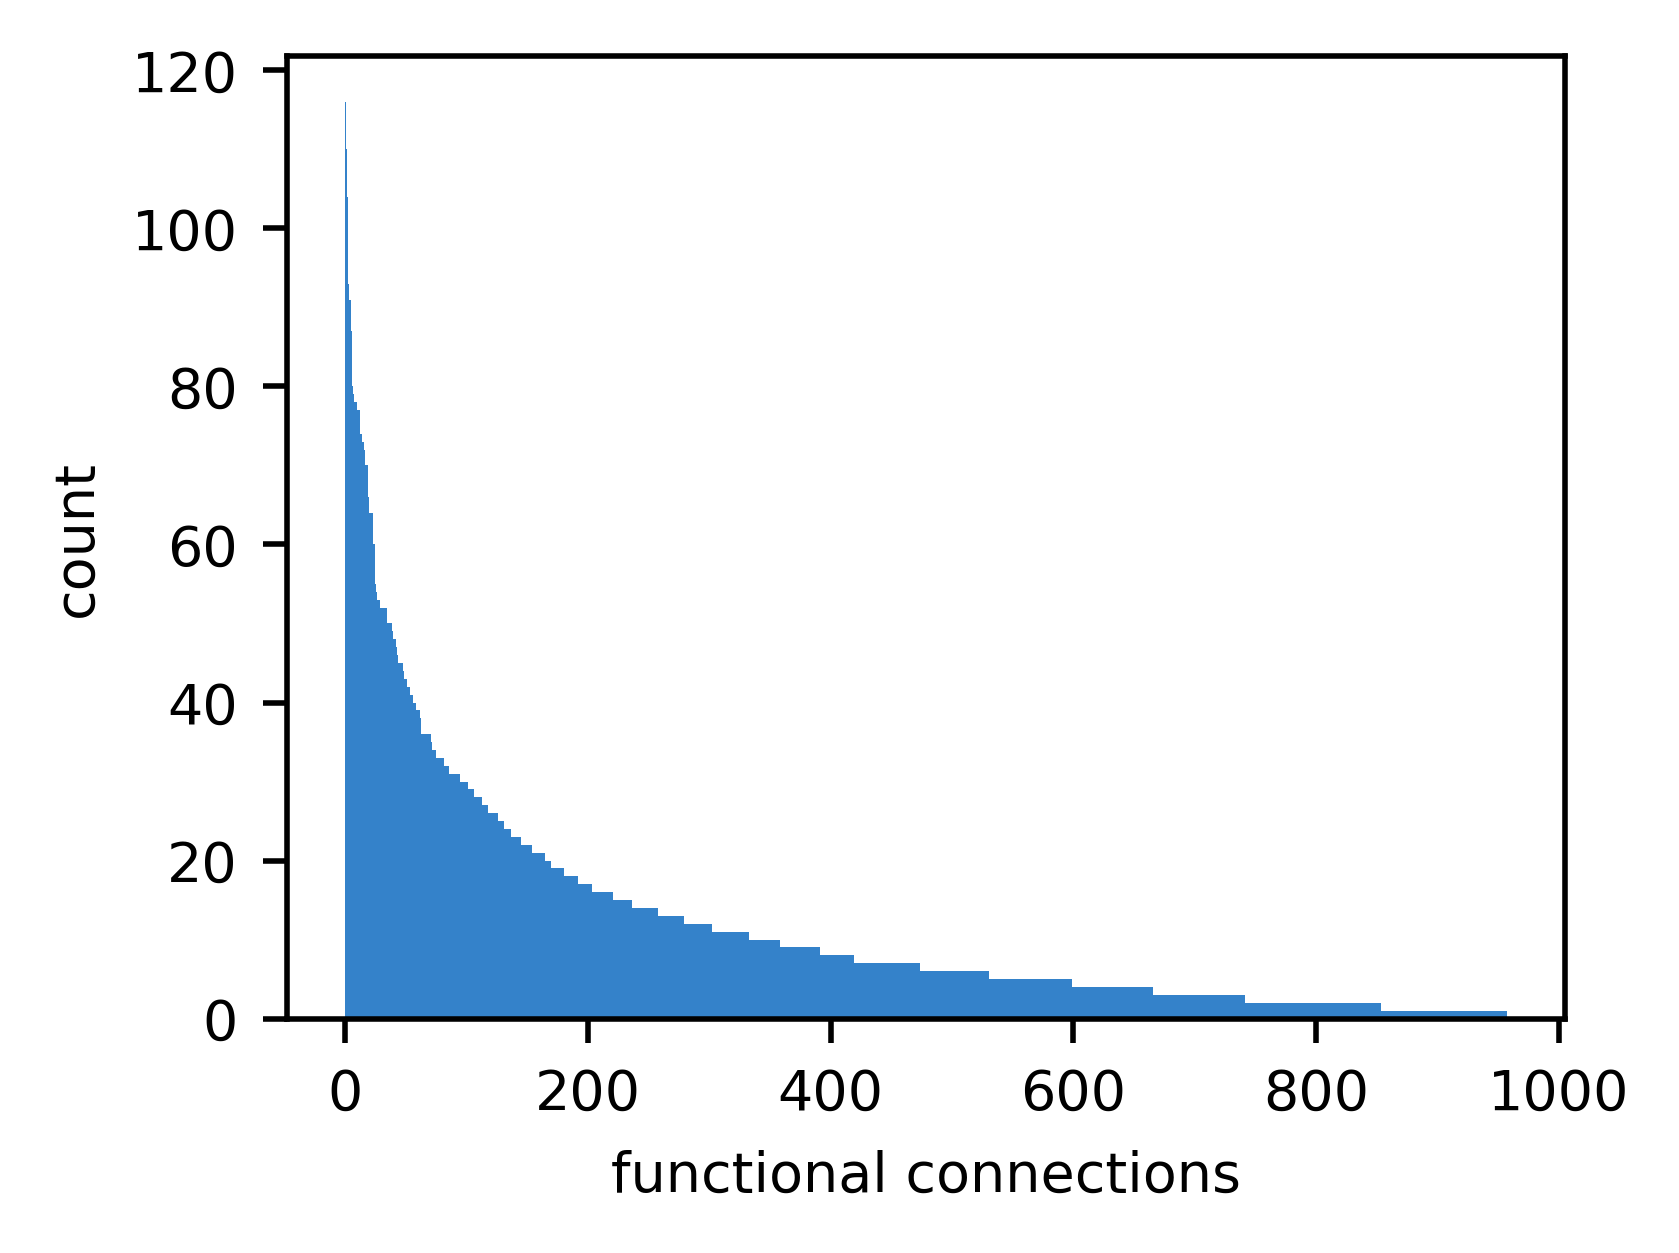
\includegraphics[]{ff.png}
	\caption{Number of times the feature appears in the top 100 of each window}
\end{figure} 

We tallied the number of times that each feature ranked in the top 100 in $N$ windows($N$=116 in our paper). The number of times each feature appears in the top 100 is shown in Figure 2. With only 13 features appearing more than 66.7\% of the time, it is evident that functional brain connection is sparse. After considering the average ranking of these features, we finally picked 30 features for presentation.The brain projection maps of all 30 functional connections and the projection maps of important brain regions are shown in Figure 3, and the top 10 are shown in Table 6.
\begin{figure*}[h]
	\centering
	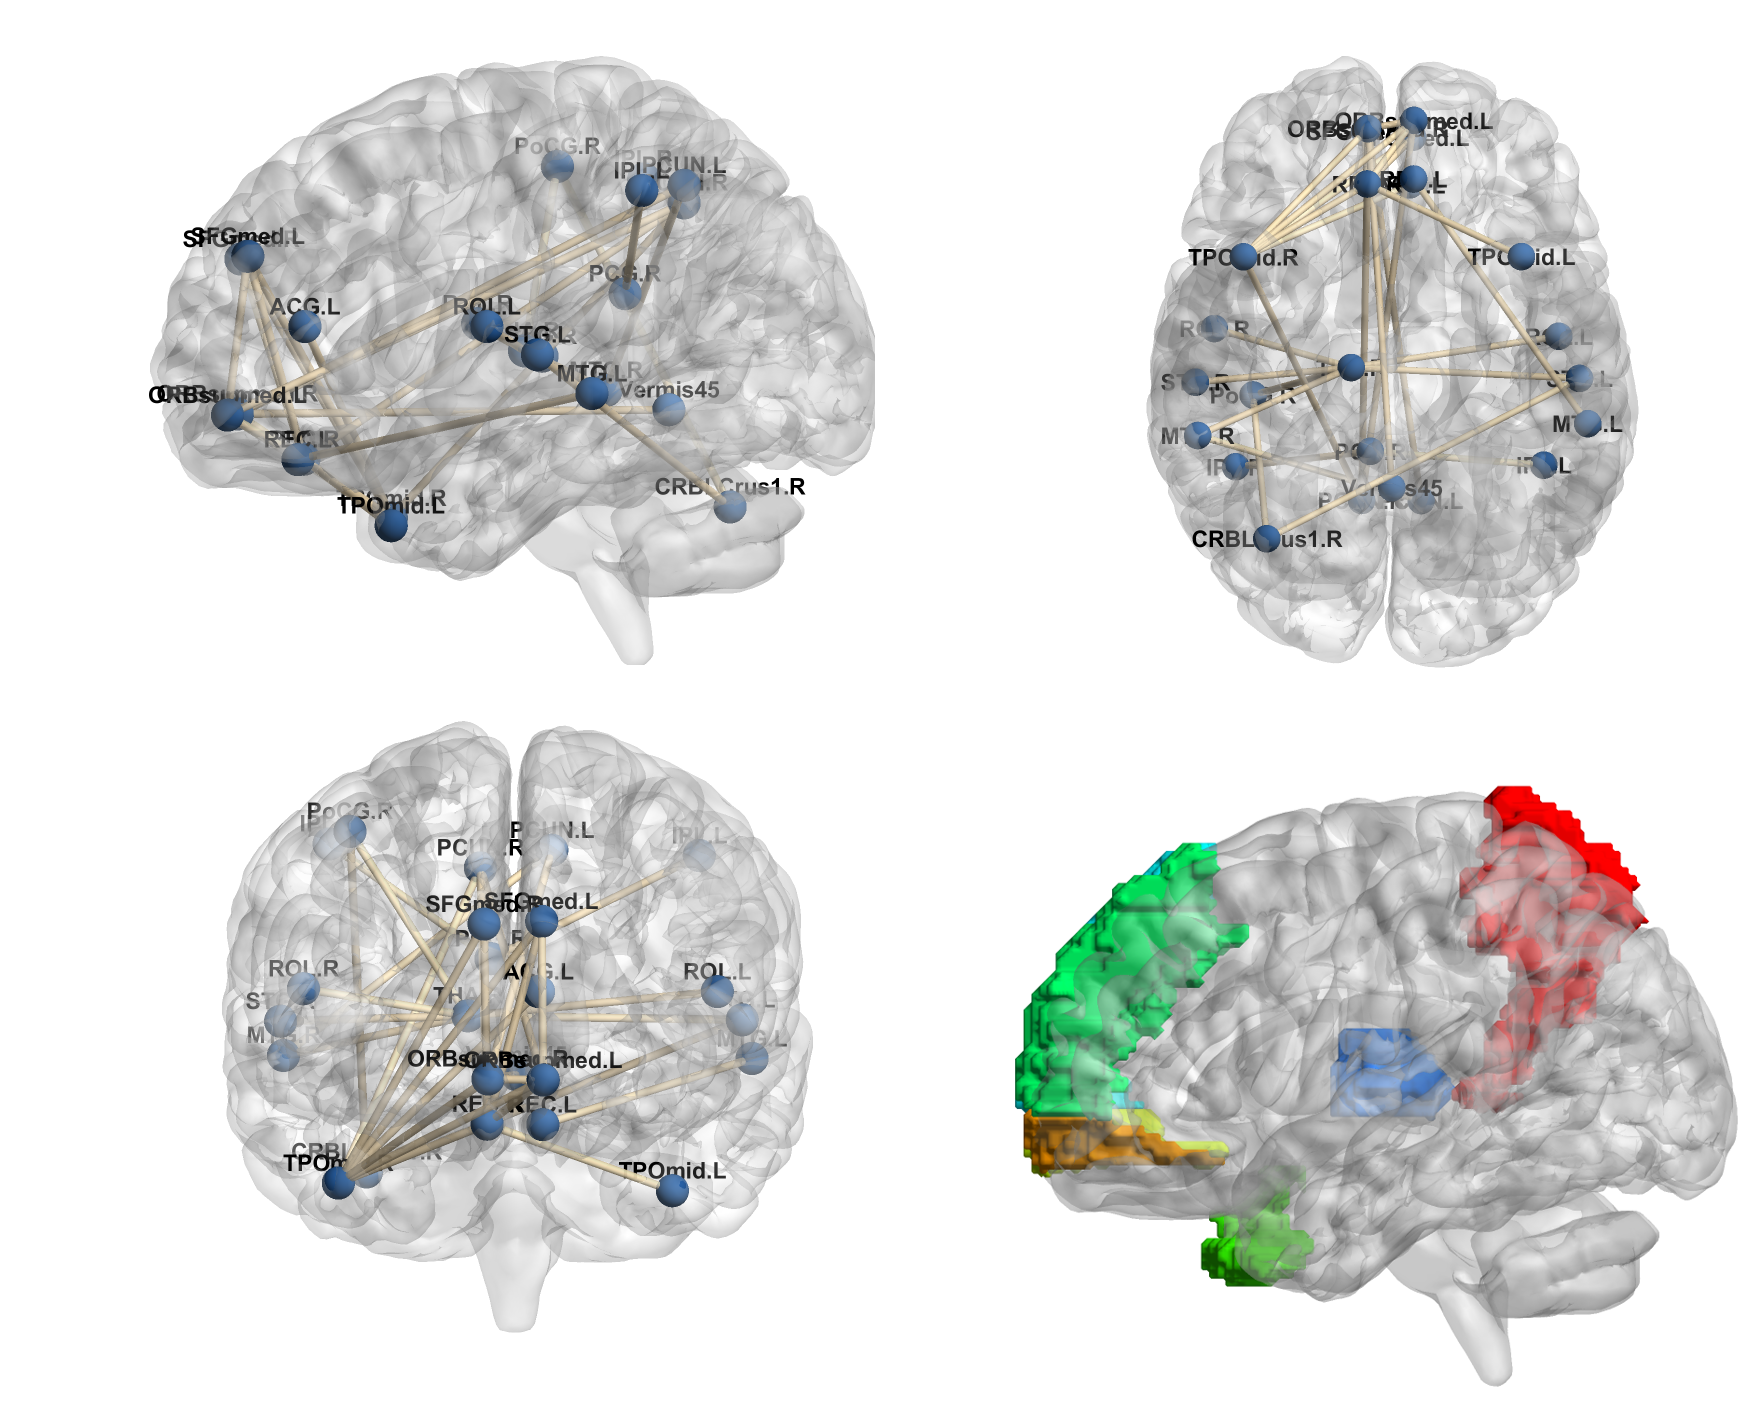
\includegraphics[scale=0.4]{brain.png}
	\caption{Projection of the top 30 most discriminative functional connections in the brain}
\end{figure*} 
Superior frontal gyrus and  (particularly FrontaI Sup Media in AAL) and middle temporal gyrus (particularly TemporalI PoIe Mid in AAL) were found to have a substantial effect on ASD. In terms of functional connectivity, Cingulum Ant and TemporaI Pole Mid were the only functional connections that appeared in all windows. Connections between Frontal Sup Medial and Rectus, Frontal Mid 0rb and Precuneus also appeared in almost all windows. Additionally, the relationship between the thalamus and temporal lobe arises frequently and is noteworthy. Similar results have been obtained in previous studies(refer).

\begin{table*}[]
	\tabcolsep=1cm
	\caption{10 brain connections most likely to cause ASD}\label{Table6}
	\begin{tabular*}{\tblwidth}{@{}ccccc@{}}
		\toprule
		\textbf{ID} & \textbf{ROIs}      & \textbf{\textbf{Hemisphere}} & \textbf{\textbf{ROIs}} & \textbf{\textbf{\textbf{\textbf{Hemisphere}}}}  \\  % Table header row
		\midrule
		1                               & Cingulum Ant       & L                            & TemporaI Pole Mid      & R                                               \\
		2                               & Frontal Mid 0rb    & R                            & Precuneus              & R                                               \\
		3                               & Frontal Sup MediaI & L                            & Rectus                 & R                                               \\
		4                               & Postcentral        & R                            & Thalamus               & R                                               \\
		5                               & TemporaI Sup       & L                            & Thalamus               & R                                               \\
		6                               & Frontal Mid 0rb    & L                            & Frontal Mid 0rb        & R                                               \\
		7                               & FrontaI Sup Medial & R                            & Rectus                 & R                                               \\
		8                               & FrontaI Sup Medial & R                            & TemporaI Pole Mid      & R                                               \\
		9                               & Thalamus           & R                            & TemporaI Sup           & R                                               \\
		10                              & FrontaI Sup Medial & L                            & TemporaI PoIe Mid      & R \\
		\bottomrule
	\end{tabular*}
\end{table*}
\section{Discussion}
In this paper, we partition the time series into numerous overlapping and independent windows using sliding windows. For each window, a functional connectivity vector is constructed using the Pearson correlation coefficient, and the functional connectivity vectors are combined to generate dynamic functional connectivity. Compared to the widely used static functional connectivity, dynamic functional connectivity captures fluctuations in the temporal dimension of the BOLD signal. However, it also exacerbates the conflict between small sample size and high dimensionality, so feature extraction is essential.

We use Kendall's rank correlation coefficient for feature extraction. This method selects features with high discriminative power without changing the raw data, and all operations are done before the model training, which largely reduces the time required for model training. The final results demonstrate that the model achieves the highest performance when 1024 features are chosen for training, which demonstrates the sparsity of the brain functional connectivity network and demonstrates the importance of feature extraction in relevant research. How to select more discriminative features is a crucial prerequisite for achieving excellent model performance.

We added positional encoding to the input data because the self-attention mechanism lacked the ability to model temporal order. This encoding method accurately depicts the input order of the windows without increasing the amount of model parameters, making it easier for the model to capture variations in nearby windows. The multi-head self-attention mechanism is exceptional at gaining global information, whilst the numerous heads enable the model to acquire knowledge from several subspaces. We also employ feed forward neural networks to get feature combinations in higher-dimensional spaces and to eliminate feature combinations with low discrimination by recovering the preceding dimension. Residual networks help decrease gradient disappearance and accelerate model training. Our model achieves an average accuracy of 76.22\% and an AUC of 0.8132 when subjected to ten-fold cross-validation. Additionally, we validated the model across various sites using inter-site cross-validation, and the model's average accuracy of 76.71\% illustrates its strong generalizability. In our studies, the model worked optimally at $H$=6, demonstrating that the brain functional connectivity network includes a plethora of information. Future study should place a greater emphasis on extracting the data's abundant information, such as utilizing HOFC to define the correlation of correlations between brain areas.

Using the Kendall feature ranking, we determined the ten functional connections most likely to cause ASD. The superior frontal gyrus and middle temporal gyrus are most likely connected with the prevalence of autism. Connections between the cingulum Ant and TemporaI Pole Mid, Frontal Sup Medial and Rectus, Frontal Mid 0rb, and Precuneus were present in the majority of windows. Also essential is the relationship between the thalamus and temporal region. This serves as a resource for future studies on autistic pathophysiology.
\section{Conclusion}
In this paper, we propose a self-attention mechanism-based method for diagnosing autism. We construct dynamic functional connectivity from raw data using sliding windows, apply Kendall rank correlation coefficients for feature selection, and integrate multi-headed self-attentive layers with feed forward neural networks to discriminate ASD with outstanding results. According to the results of feature ranking, the superior frontal gyrus and middle temporal gyrus were determined to have the most significant effect on ASD. Our model contributes to deep learning for diagnosis of mental disorders and research on autism pathology.
% To print the credit authorship contribution details
%\printcredits

%% Loading bibliography style file
%\bibliographystyle{model1-num-names}
\bibliographystyle{cas-model2-names}

% Loading bibliography database
\bibliography{}

% Biography
%\bio{}
% Here goes the biography details.
%\endbio

%\bio{pic1}
% Here goes the biography details.
%\endbio

\end{document}

